\documentclass{article}
\usepackage{graphicx}
\usepackage{amsmath}
\graphicspath{ {files/RCP_diagram/} {files/}}

\title{Multi-Scale Resolution of Human Social Systems:  A Synergistic Paradigm for Simulating Minds and Society}
\author{Mark G. Orr}

\begin{document}
\maketitle

\section{Introduction}
Recently, we put forth an initial sketch of what we call the \textit{Resolution Thesis}\cite{orr2018_brims}.  The thesis holds that 1) models of cognition will be improved given constraints from the structure and dynamics of the social systems in which they are supposed to be embedded, and 2) the resolution of social simulations of agents will be improved given constraints from cognitive first principles\footnote{Cognition considered as theoretical models of human perception, thought and action that includes, broadly, explanations of emotion, motivation, and affect in addition to more tradtional domains of cognitive psychology and cognitive science; one could arguably use the term \textit{psychological first principles} as equivalent}.  This thesis reflects a variety of motivations, the most obvious being the observation that there is little overlap between the cognitive sciences and the generative social science approach[*REF EPSTEIN, 2008], both of which rely heavily on computer simulation to understand aspects of human systems, albeit different aspects of human systems with respect to scale.  The former focuses almost exclusively on the mind as a scientific object of study for which the lion's share of simulation efforts reflect a normative mind (one mind at a time, non-social or statically social) and the latter emphasizes multiple aspects of social systems, the mind being only one of these aspects.  For this latter case,  there is little relation to the vast experimental evidence of how the mind operates or what are the central theoretical entities that compose the mind.  To a large degree, the resolution thesis is a recognition that an interdependence between cognitive science and generative social science has yet to be leveraged for the purposes of improving our understanding of both.    

The Resolution Thesis can be understood from multiple perspectives.  From the view of cognitive science, the thesis means that patterns of organization (e.g., information flow on the internet [REF; FROM SOCIALSIM], clustering of behaviors in a community[REF CHRISTAKIS]) at the social and organizational level should inform cognitive models.  In other words, when possible, these patterns should be included as convergent evidence for a theory or model.  Although it is desirable for cognitive models that are implicated in social behavior to have some reasonable explanatory scheme that links facets of the cognitive model to aspects of social organization, this is rarely the case.  (Anderson's Relevance Thesis, a rare exception, reasons about how cognition may have implications for social organization.)  The reader might notice that it is difficult to think about using social organization as part and parcel of the convergent evidence of a cognitive model without first considering the implications of cognition for social behavior.  But that is precisely the point--it is natural, once of the mind to think about how cognition scales to social systems, to think about using the degree to which it scales accurately as part of the convergent evidence for having confidence in the model. 

From the generative social science perspective, the Resolution Thesis means that the representations of agents should be informed closely by cognitive science and relevant neurophysiological considerations.  This runs somewhat counter to the principled adherence to simplification of the internal processing of simulated agents found in this literature, one that, in fact, served to show that complex social dynamics can be driven by simple behavioral rules of agents.  However, more recently, there are efforts in the generative social sciences that acknowledged that closer ties to the psychological and neurophysiological underpinnings of human behavior may yield benefit.  Epstein's neurocognitive approach is a notable effort in this vein[REF, Epstein 2014]; there are other related approaches (e.g. REF 19-22 from BRiMS).  These efforts notwithstanding, there remains a large gap between them and the implementation of models from cognitive science and psychology, not necessarily in principle, but in practice. [DO WE MENTION HERE THAT THE SUN AND VAN OVERWALL GROUPS HAVE CALLED FOR COGNITION TO GROUND SOCIAL SCIENCES FOR AT LEAST A DECADE, PROBABLY SHOULD]


A third and more general view is that the Resolution Thesis is about human systems for which the distinction between neural, cognitive and social levels of scale should be considered counter-productive.  An understanding of any of these levels of scale is dependent, to some degree, on an understanding of the others.  In effect, the notion of convergent evidence as originating, in part, from other levels of scale, applies to all levels of scale.  The implication is that we should leverage information across scale in an iterative and synergistic way, if not simultaneously. 

The Resolution Thesis, despite sounding both reasonable and practical at face value, is opposed by reasonable argument from both the cognitive sciences and generative social sciences.  Simon's notion of nearly decomposable systems--that the temporal dynamics of adjacent levels of scale, in most systems, are little correlated--suggests that we can understand well the dynamics at each level of scale independently of the others(*REF, SIM 1962; see P. Anderson, 1972, for similiar argument in phyical systems).  The KISS principle (keep it simple, stupid) used heavily in the generative social sciences, is clearly akin to Simon's notion, and is bolstered by its early wins in understanding the behavior of social systems using simple, non-cognitive agents (REF 15-17 from BRIMS).  In cognitive science, Newell, in considering the time scale of human behavior, suggested that the social band ($> 10^4$ seconds, representing social systems and organizational behavior) is characterized to be weak in strength in the sense that it may not provide computations in a systematic way (relative to lower temporal bands, e.g., cognitive and neural processes).  

These counter arguments notwithstanding, our working assumption is that the degree to which the  \textit{Resolution Thesis} is useful is an empirical issue.  The state of the art in technology, computing and the their tight coupling to the current social mileau affords, we think, the testing of the Resolution Thesis.   To this end, we've developed the \textit{Reciprocal Constraints Paradigm} (henceforth \textit{RCP}), a methodological approach that might lay a foundation for fruitful social simulation and an understanding of the implications for theory and models across levels of scale.


\section{The Reciprocal Constraints Paradigm}
The value of the \textit{RCP} does not lie in precise formal presecription, but in providing a scaffold for building understanding of social systems, and, possibly providing a deep understanding of the interdependencies among levels of scale.  Further, the \textit{RCP} was conceived when considering multi-agent systems and cognitive science where human behavior, in both cases, is implemented in a simulation enviorment in which agents are represented algorithmically.  This is not meant to preclude other methods and approahces (e.g., analytically tractable economic games), but just to provide the context for the development of the ideas presented here.

\begin{figure}
	\centering
	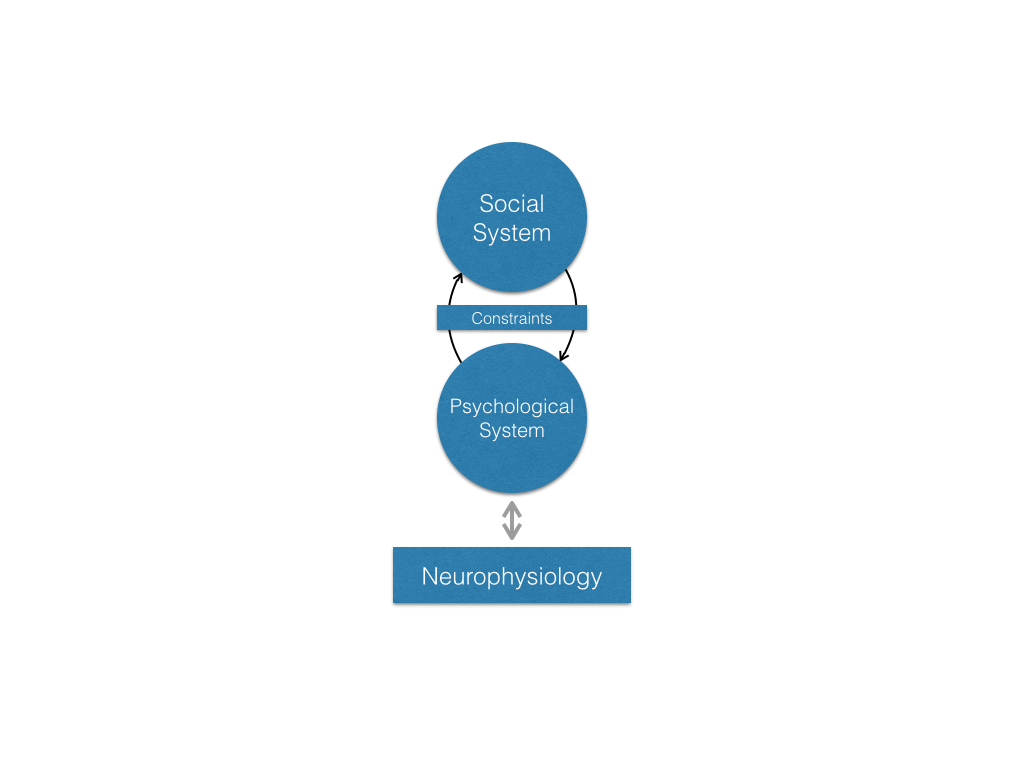
\includegraphics[width=1.0\textwidth]{RCP_diagram.png}
	\caption{\label{fig:rcpdiagram} The four components of the \textit{RCP} are a cognitive system, a social system, and the constraints on each one from the other.  In the \textit{RCP} social systems and cognitive systems are assumed to be derived from and exhibit an abstract set of first principles \& properties, called $S$ and $C$, respectively.  Also captured here is the potential for integrating neurophysiolgical considerations into the cognitive system when appropriate; these may prove as essential for some social systems (the grey two-headed arrow indicates this potential). The notion of constraint refers to the use of information from $S$ \& $C$ to inform one another in a principled way.  
	}
\end{figure}

Figure \ref{fig:rcpdiagram} shows the four primary components of the \textit{RCP}: a cognitive system, a social system, and the constraints between levels of scale.  We assume that social systems and cognitive systems are derived from and exhibit an abstract set of first principles \& properties, called $S$ and $C$, respectively (e.g., theoretial entities, experimental paradigms, patterns in empirical data in respect to the discipines that address a particular level of scale).  Further, defining $S$ and $C$ will depend on the social system or cognitive system of interest.  The notion of constraint simply refers to the use of information from $S$ \& $C$ to inform one another in a principled way. An upward-constraint refers to information from $C$ informing $S$; downward-constraints reverse this relation.

 A primary example in $C$ is the set of allowable algorithms $A$ such that $a \in C$ with grounding in empirical work in cognitive science and psychology.    Primary examples in $S$ are the social structures, channels of information, and dynamics that characterize a social system, much of which is formalized using graph theory/network science.    It is important to emphasize that within $S$ are notions regarding the behavior of agents, not only social structures.

A central assumption in the RCP is that cognitive systems and definitions of agent behaviors in social systems are meant to represent human information-processing capacities that can be described as mathematical functions. \cite{van Rooij, 2008}\footnote{This is equivalent to Marr's computational level; we will use Marr's computational, algorithmic, and implementation levels of description\cite{Marr,1981} throughout this paper.}. Thus, in $C$ we can define a cognitive system as $\psi_{ct}: I_{ct} \rightarrow \psi_{ct}(i)$ where $I_{ct}$ is the set of allowable inputs and $\psi_{ct}(i)$ is the output; in $S$ we have a corresponding agent definition as $\phi_{at}: I_{at} \rightarrow \phi_{at}(i)$ where $I_{at}$ is the set of allowable inputs and $\phi_{at}(i)$ is the output for an agent\footnote{Social and cognitive systems may define parameters regarding variability among a set of agents; this is not reflected here.}. 

\subsection{Applying the Reciprocal Constraints Paradigm}   
In practice there are multiple approaches available for application of the RCT, but what unites them is the study of a human social phenomena, either defined at one level of scale or at multiple levels of scale.  Naturally, the first step is to identify a social phenonmena of interest, a task that is inherently tied to one's perspective.  If the perspective is largely in $C$, then the focus would most likely be on understanding the psychological processes, representations, etc. in relation to social systems, but informed in some way by $S$.   Another perspective, largely in $S$, would dictate a concern with the social structures and dynamics of the social system (multiple humans interacting) with some degree of constraint from $C$.  These two perspectives are both what we call single-scale approaches to the \textit{RCP}. Of course, one could take a multi-scale perspective that treats $C$ and $S$ simultanteously. This perspective likely depends on a simulation approach that captures aspects of $C$ and $S$ in one runnable system.  

These two approaches are different, primarily, in terms of the directness of the constraints.  Single-scale approaches use information that exists prior to application (in any form it can get it); multi-scale generates simulated information at each level of scale, which, also exists prior to application.[NOT SURE IF WE KEEP THIS IDEA] 

We will address the obvious issues and difficulties in applying the \textit{RCP} after providing a description of some potential methods for application.  The goal in this section is simply to express what it might look like to apply the \textit{RCP}.   

\subsubsection{Single-Scale Approaches}
It is conceivable that a fruitful applcation of the RCP might occur at one level of scale.  Let us first consider the cognitive level of scale.  There exists a large literature on neural and cognitive approaches to understanding human social behavior and social psychology\footnote{Division 8 of the American Psychological Association is dedicated to social psychology} with the requisite broad range of methods and theoretical orientations, so defining a social phenomena of interest is natural at the cognitive level. One potential approach, then, for implementing the \textit{RCP} would be to map general properties of cognitive systems with properties of social systems.  For example, a central finding in cognitive science and psychology is that learning mechanisms are sensitive to the order in which information is presented to the system (e.g., a human or computational model of a human).  Further, there is a large set of social phenomena that imply some type of learning mechanism (attitude formation [REF ORR]; impression formation [REF MONROE]).  Thus, we can conclude, reasonably, that order matters for some social phenomena at the psychological level.  The application of the RCT, in this case, means inferring what a distribution of the temporal order of inputs would be given some $s \in S$ . (This distribution, almost axiomatically, seems dependent upon some propoerties of $S$ if $S$ contains graph $G$ where $V(G)$ and $E(G)$ are the agents and information channels, respectively.)  Off-hand, there seem to be candidate examples from the literature regarding human socio-technical networks(e.g., [REF BEARMAN; REF BARABASI WEB]), but what this means precisely would depend on the social phenomena of interest (e.g., early language development may depend on a different $G \in S$ compared to racial stereotypes).  

At the social level of scale, an obvious approach is an analysis of the degree to which $\phi_{at}$ compares to any $\psi_{ct} \in C$.  For the case in which $\phi_{at}$ and $\psi_{ct}$ are formally well defined, this might be relatively straigtforward\footnote{Potential methods for such a comparison would, idealy, focus not only comparison of input/output functions but also the nature of the runnable algorithm}.  But, there will certainly be cases for which this is not true.  For example, imagine that $\psi_{ct}$ is only defined in terms of an experimental paradigm, theoretical apparatus and the interpetation of data resulting from application of the experimental paradigm\footnote{Some might argue that under these conditions, the notion of a functional mapping $\psi_{ct}$ is nonsensical}.  One appraoch for comparison in this case would be to explore the behavior of $\phi_{at}$ by simulating an experimental paradigm that is isomphorphic to that used to define $\psi_{ct}$ (assuming $\phi_{at}$ is defined algorithmically).  In essence, this is like running an psychological experiment on artificial agents, an approach that is akin to simulation in the psychological sciences.  The output of these experiments could be compared to the patterning and dynamics of human performance in $C$.  

 \subsubsection{Multi-Scale Approach}
The multi-scale approach is simple in principle: build a simulation platform that simultaneosly captures essentail aspects of both $S$ and $C$ (e.g., an agent-based model of cognitive agents).  In this case, the upward-constraints refer directly to the substition of $\psi_{ct}$ for $\phi_{at}$.  The downward-constraints are generated with respect to the degree to which the simulated social system matches $S$ as defined by the pheonomena of interest.  The downward constraints serve as a signal that would suggest modifications to $S$ $C$ or both.

Althought the concept is simple in principle, the detials include many decisoin points and free parameters.  Primary of these are the following. This still requires comparing the algorithms that generate $\psi_{ct}$ and $\phi_{at}$.  It also requires defining an objective function for the relation between the simulation output and some empirical data structure.  It also requires decisions, when outside some cost function tolerance, of what aspects of the system to change in order to optimize the cost function, $S$, $C$ or both.  In the case that $C$ is changed, then there are many decisions with even $\psi_{ct}$ that may be required.  

Under some conditions, this simulation approach may afford automization of its search space to reduce the error in the objective function (if computable).

\subsection{Issues in Applying the Reciprocal Constraints Paradigm }
1. Both single- and multi-scale approaches to the \textit{RCP} are fraught with difficulty in application.  

2. FREE PARAMETER PROBLEM AND Acountable modeling: 

3. What if $S$ is dependent on $C$?

4. Many competing cog models for any phenomena...Issues of the right cogntive model, lots of cog models....

5. Downward constraints in multi-scale approach....what precisly is changed

The second kind is to abstract some details from full-fledged cognitive models, but adhere to a principle of \textit{Accountable Modeling}\ref{LebiereX}.

\section{Analysis of Related Work}
Here we provide examples of prior work that employ parts of the RCP.  As we have no known examples of the downward-constraints, we focus on upward-constraints.  These are not exhaustive; we apologize for any work not mentioned, but wanted to assure the reader that there are some useful examples in the literature that speak to the feasibility of implementing the \textit{RCP}.  

\section{An Example of RCT Implemented}
Christian's sim

Note, we may just provide examples of how Stocco's work might be used in our example...not run the actual sims if not have time.

\section{Discussion}

\subsection{Moving Forward}
From the single level of scale approach, One idea is to catalog social phenomena captured by psychological models and do a mapping of $C$ to $S$. \footnote{In the limit, the social features and the cognitive features have co-evolved on an evolutionary time scale}.



  




\bibliographystyle{plain}
\bibliography{references}

\end{document}